\chapter{Results}

	\section{Static Calculation}
		The results of static calculation are shown in the following sections. Firstly the results of office building then the residential building results at each steps are shown below according the methodology. A summary is also given after each energy loss and energy gain section is presented.

		\begin{figure}[htbp]
		\centering
		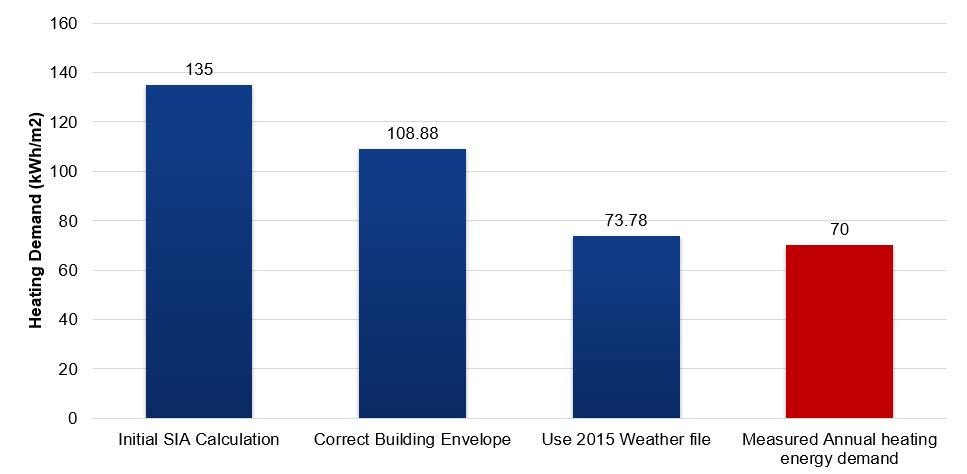
\includegraphics[scale=0.4]{Office_SIA.jpg}
		\caption{SIA Calculation Improvement for Office Building}
		\label{fig:Sumatra_SIA}
		\end{figure}
		
		\begin{figure}[htbp]
		\centering
		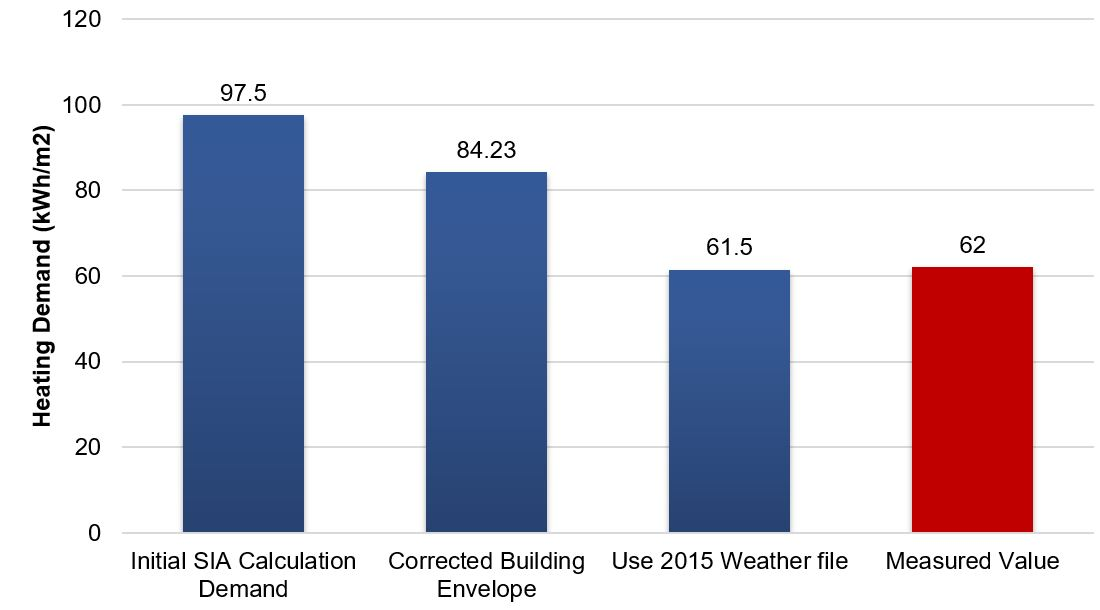
\includegraphics[scale=0.4]{Residential_SIA.jpg}
		\caption{SIA Calculation Improvement for Residential Building}
		\label{fig:Hongger_SIA}
		\end{figure}
		
		
	\newpage		  
	\section{Dynamic Simulation}		
			The dynamic simulation results are shown below in Figure \ref{fig:Sumatra_EP} and Figure \ref{fig:Hongger_EP} below. Firstly, the simulation is run in 2015 weather conditions and with standard building envelope. Secondly, the air change ratio is changed to a more realistic value of 0.3 ACH. Then, the SIA standard heat convection coefficient values are applied on the model and the result shows a close match between the calculated heating demand and the measured heating demand. It appears that both buildings can obtain a very close estimation when using these approaches. However, in order to further verify the building simulation methods and parameters, a building calibration is needed for both buildings.
		

		\begin{figure}[htbp]
		\centering
		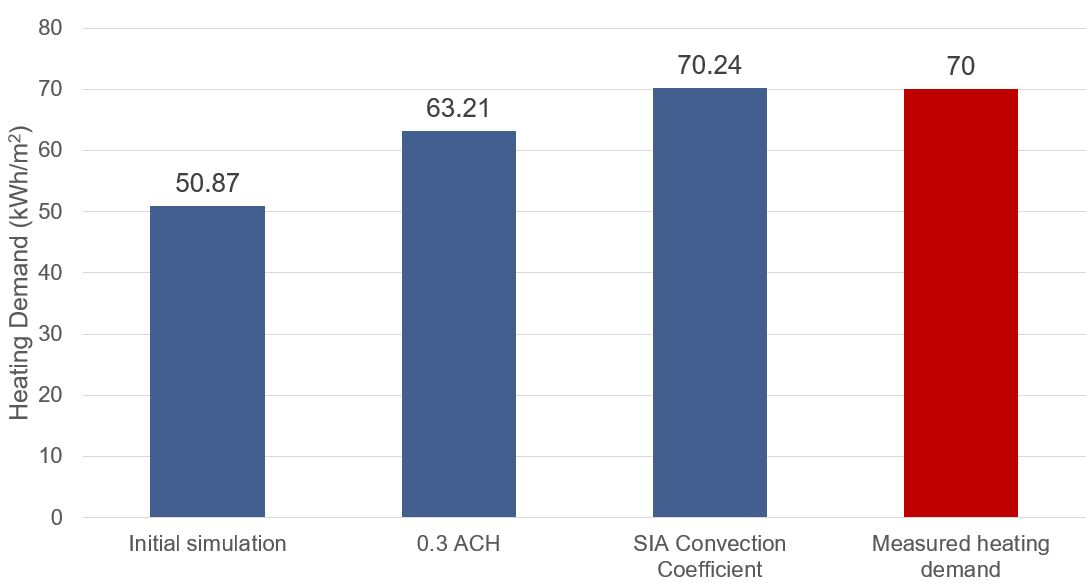
\includegraphics[scale=0.5]{Office_EP.jpg}
		\caption{Office Building Dynamic Calculation Correction}
		\label{fig:Sumatra_EP}
		\end{figure}

		\begin{figure}[htbp]
		\centering
		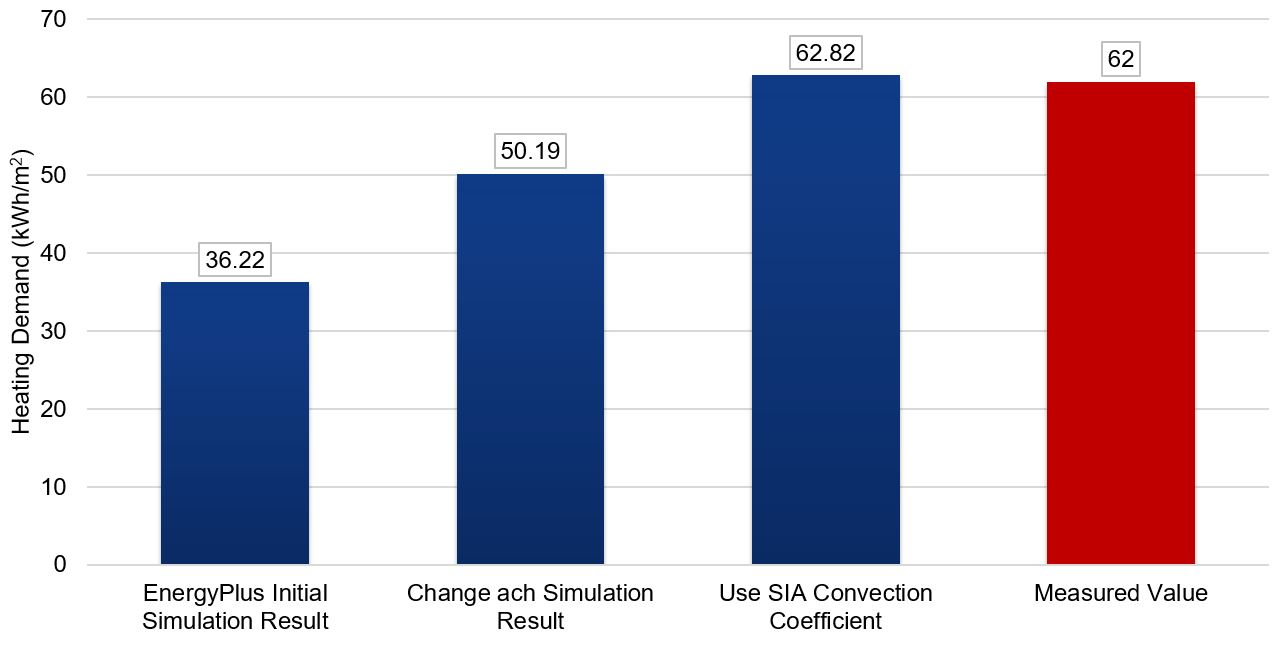
\includegraphics[scale=0.4]{Residential_EP.jpg}
		\caption{Residential Building Dynamic Calculation Correction}
		\label{fig:Hongger_EP}
		\end{figure}
		
		




	\section{Calibration Results}

			Figure \ref{fig:ACH_Compare} below shows a comparison of calculated indoor temperature from 1$^{st}$ June to 10$^{th}$ June in 2015 in the residential building under different air tightness (0.1/0.3/0.5 air change per hour infiltration level). The blue line with huge fluctuation represents the outdoor temperature from the weather station, the red line represents the measured indoor temperature, and the gray, orange, and dark blue line represent the calculated indoor temperature of the three rooms at the same apartment. The result indicates that the air infiltration dose not have a strong impact on indoor temperature profile. Therefore, the air infiltration is used to calibrate the annual heating demand to the measured value after the temperature profile is matched.\\
		
			\begin{figure}[H]
			\centering
			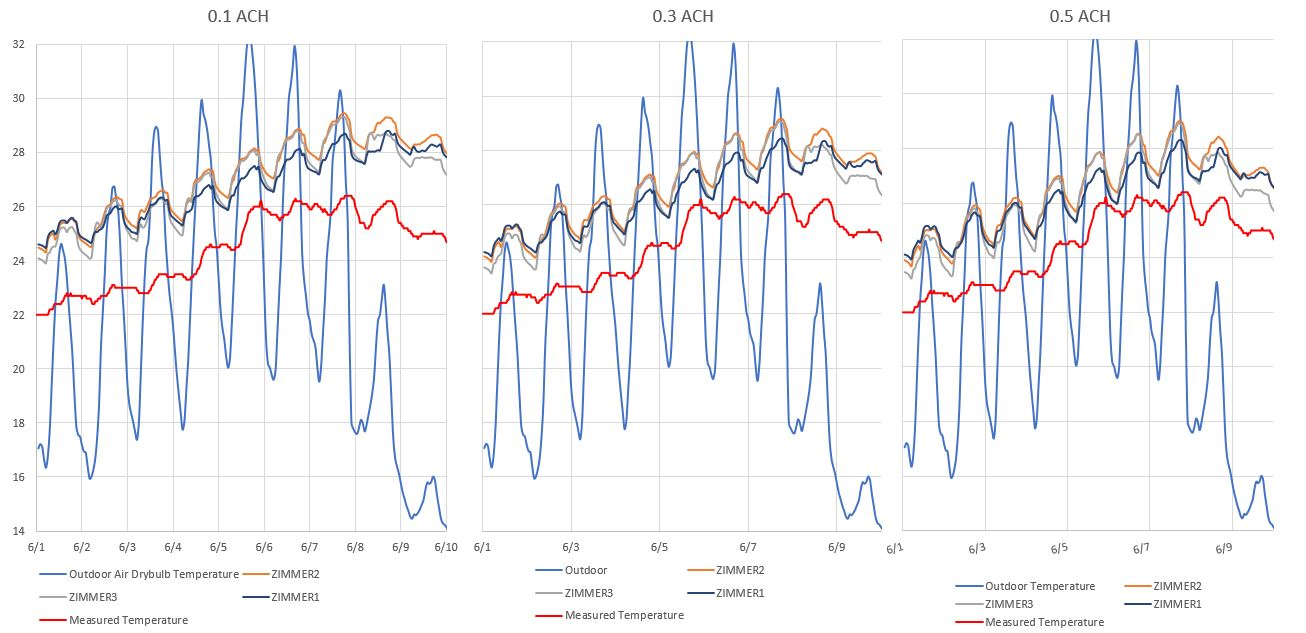
\includegraphics[scale=0.4]{ACH_Compare.JPG}
			\caption{Origin Temperature Profile of Residential Building}
			\label{fig:ACH_Compare}
			\end{figure}

			\begin{figure}[H]
			\centering
			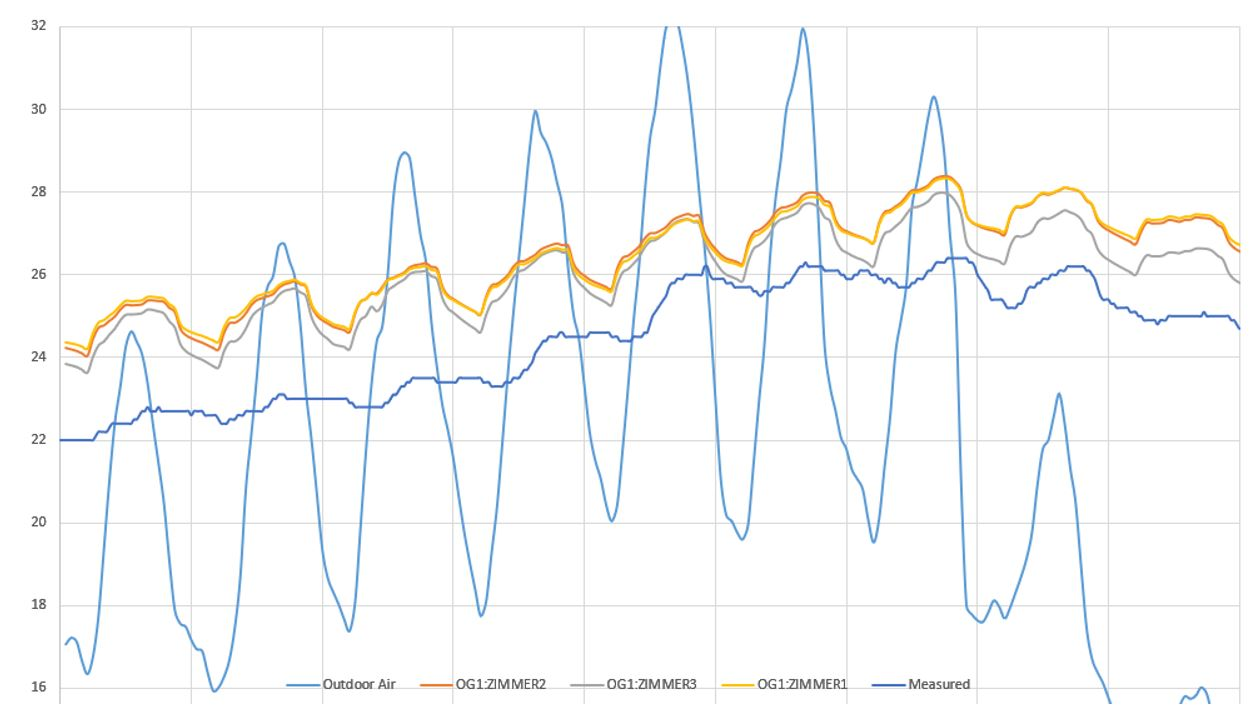
\includegraphics[scale=0.4]{Figure/Hongg_Clibration_Origin.JPG}
			\caption{Origin Temperature Profile of Residential Building}
			\label{fig:HonggCalibrationOrigin}
			\end{figure}
			
			Figure \ref{fig:HonggCalibrationOrigin} above shows a temperature profile of the first floor apartment with 0.3 ACH infiltration. The light blue line with huge fluctuation is the outdoor temperature measured by the weather station. The The less fluctuated dark blue line represents the measured indoor temperature. The rest lines in grey, yellow and red represent the calculated indoor temperature of three bedrooms within the apartment. This origin temperature profile indicates an over-estimation on heat gains. Therefore, the calibration process aimed on reducing the internal gains by varying the building appliance schedules.\\
			
			\begin{figure}[H]
			\centering
			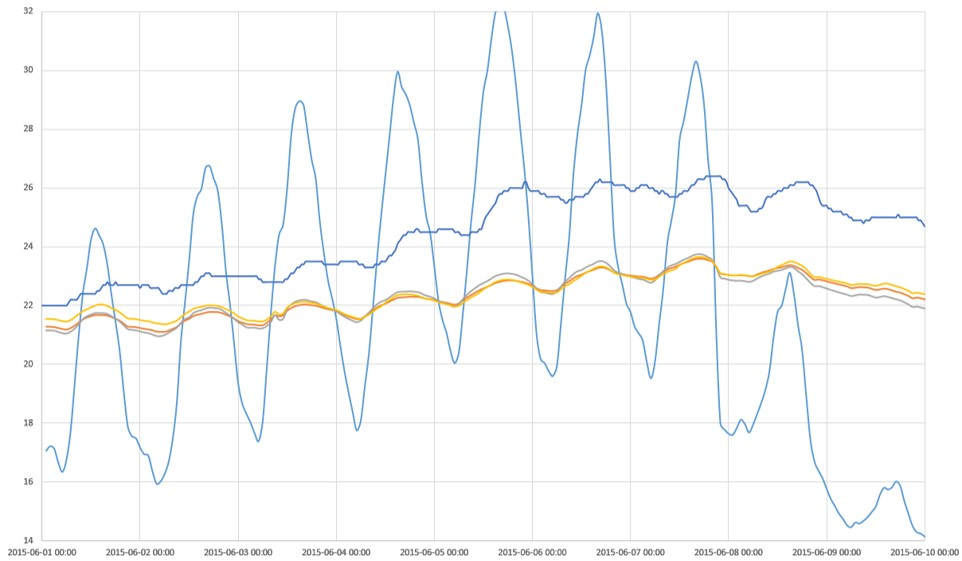
\includegraphics[scale=0.4]{Figure/Hongg_Cali_NoFacility.JPG}
			\caption{Temperature Profile of Residential Building Without Internal Gains}
			\label{fig:HonggCalibrationNoGains}
			\end{figure}
			
			In order to verify the above conclusion, another simulation is taken with no active appliance. The result in Figure \ref{fig:HonggCalibrationNoGains} proved that the wrong appliance assumption schedule is the cause of this over-heating problem. The room temperature dropped around 4 degrees when all the appliances are turned off. From the SIA 2024 schedule, the lighting schedule and lighting level for residential buildings are modified as it shows an over-estimation during daytime. \\

			\begin{figure}[H]
			\centering
			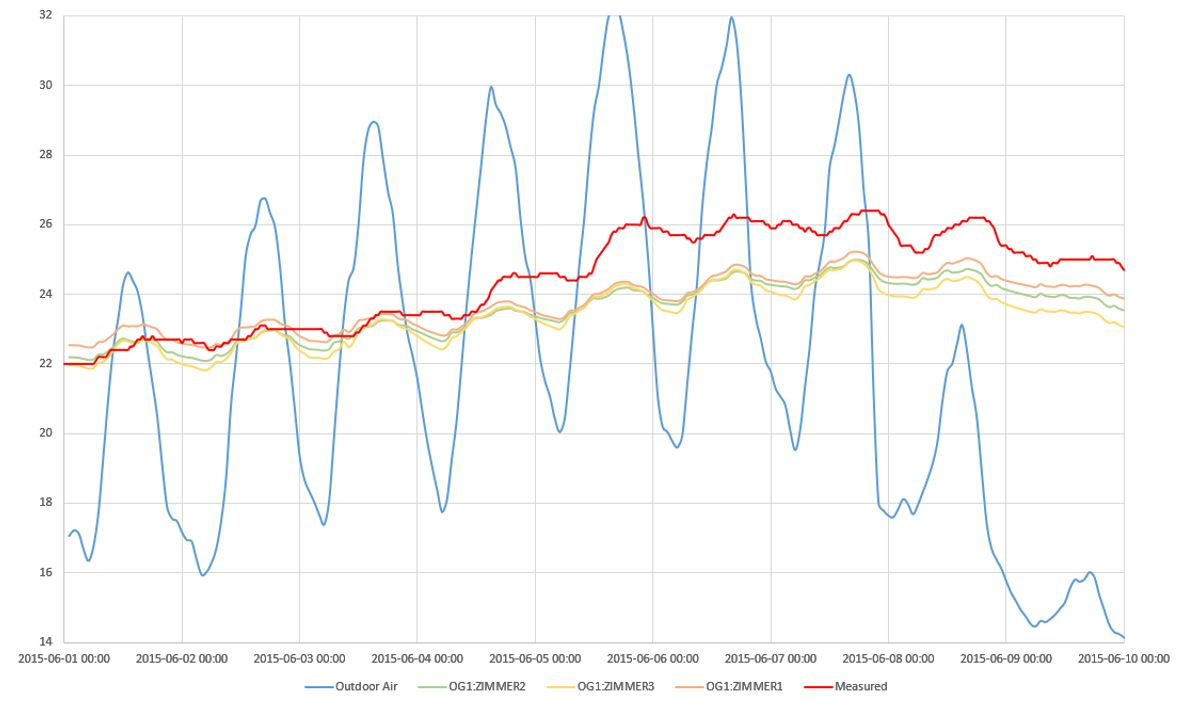
\includegraphics[scale=0.4]{Hongg_Clibration_03NoLight.JPG}
			\caption{Temperature Profile of Residential Building with No Lighting}
			\label{fig:HonggerCalibrationNoLight}
			\end{figure}

			Figure \ref{fig:HonggerCalibrationNoLight} above shows the temperature profile without lighting. The highly fluctuated blue line represents the outdoor temperature, the red line represents the actual measured data, and the orange, yellow, and light green lines represent  the calculated indoor temperature of three rooms. The result again indicated that the lighting schedule is the main cause of over-heating. Therefore, a new lighting schedule is created and rerun the simulation under a new lighting schedule. The new lighting schedule can be found in Table \ref{tab:HonggLightingCtrl} below.
			
        	\begin{table}[htbp]
        	\centering
        	\caption{New Lighting Schedule}
        	    \begin{tabular}{ccc}
        	    \toprule
        	    Lighting Schedule & Weekday & Weekend\\
        	    \midrule
                Until 02:00 & 0.05 & 0.05 \\
                Until 06:00 & 0.03 & 0.03\\
                Until 09:00 & 0.5 & 0.3\\
                Until 17:00 & 0.2 & 0.2\\
                Until 22:00 & 0.7 & 0.7\\
                Until 22:00 & 0.7 & 0.7\\
                Until 24:00 & 0.2 & 0.5\\
        	    \bottomrule
        	    \end{tabular}%
        	  \label{tab:HonggLightingCtrl}%
        	\end{table}%			
			
			
			\begin{figure}[H]
			\centering
			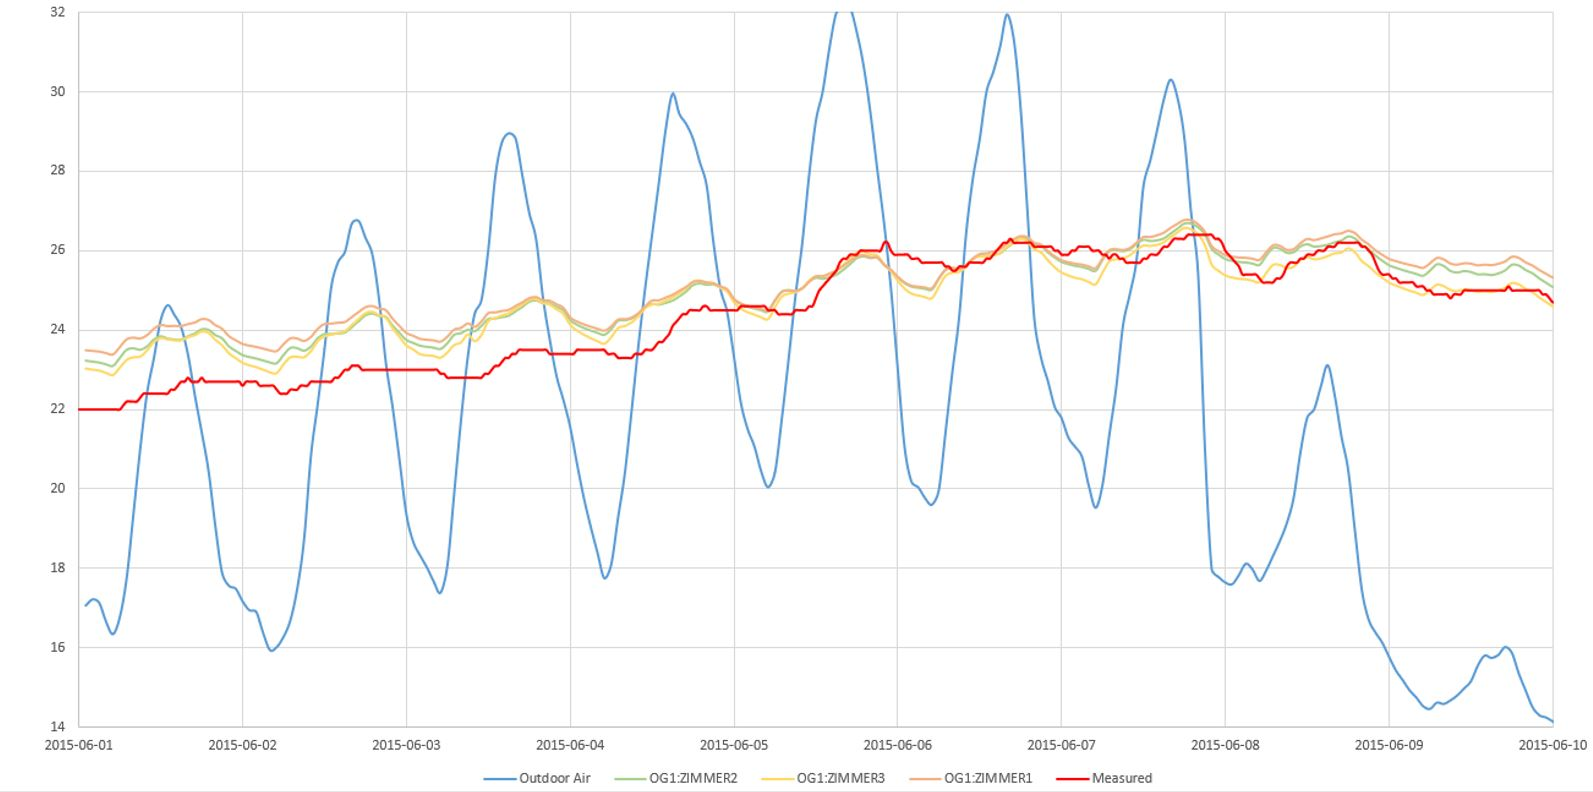
\includegraphics[scale=0.3]{Hongg_Clibration_03NewLight.JPG}
			\caption{Temperature Profile of Residential Building with New Lighting Schedule}
			\label{fig:HonggerCalibrationNewLight}
			\end{figure}
			
			From Figure \ref{fig:HonggerCalibrationNewLight} above it is known that
			The origin air infiltration level is 0.3 ACH. However, the annual heating demand indicates that this setting has higher demand than the measured value. Therefore, the air infiltration is slightly decreased to 0.25 ACH in order to fit the annual heating demand.\\ 

			\textbf{Office Building Calibration}\\
			Similarly, the office building went through a calibration process with the same approach. Firstly, the simulation is taken without any modification. An overheating is observed from the temperature profile. As the building is mostly covered with window on the west and south side, applying shading control would probably solve the problem. To test the effect of window shadings, another simulation is done under 24/7  on shading schedule. The results in Figure \ref{fig:Sumatra_Calibration_Allshade} indicates that the shading of the actual building is mainly on, as the calculated temperature profile behaved very similar with the measured temperature profile. Therefore, it can assume that the blinds at the office building is mainly on at non-heating period. While in winter period, a modest blind control is applied and the annual heating demand is observed.

			\begin{figure}[H]
			\centering
			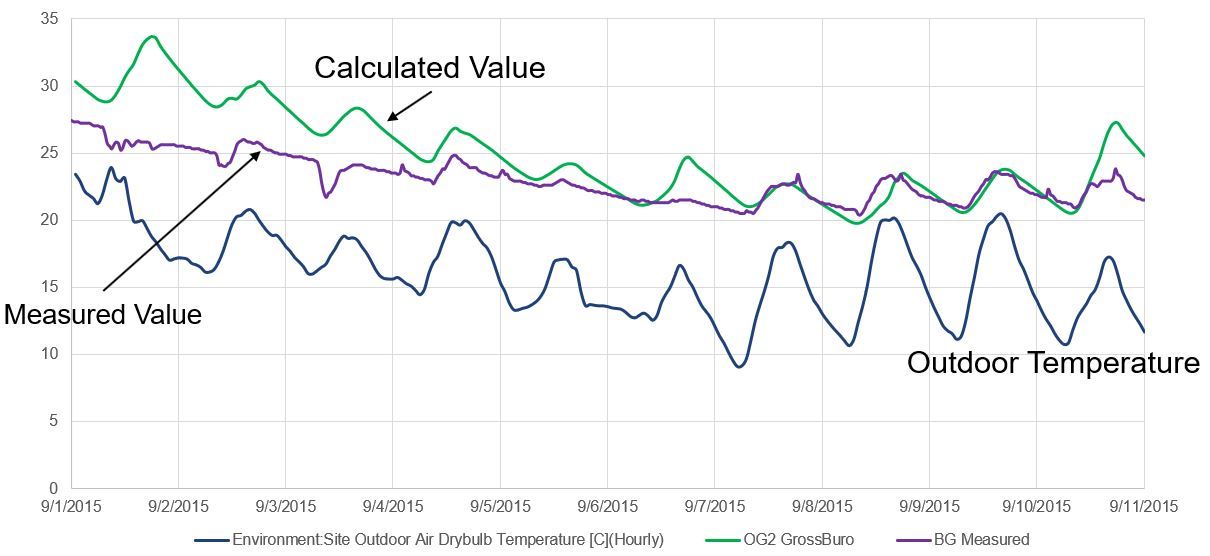
\includegraphics[scale=0.35]{Figure/Office_Calibration_Ori.JPG}
			\caption{Origin Temperature Profile of Office Building}
			\label{fig:Sumatra_Calibration_Ori}
			\end{figure}
			
			\begin{figure}[h!]
			\centering
			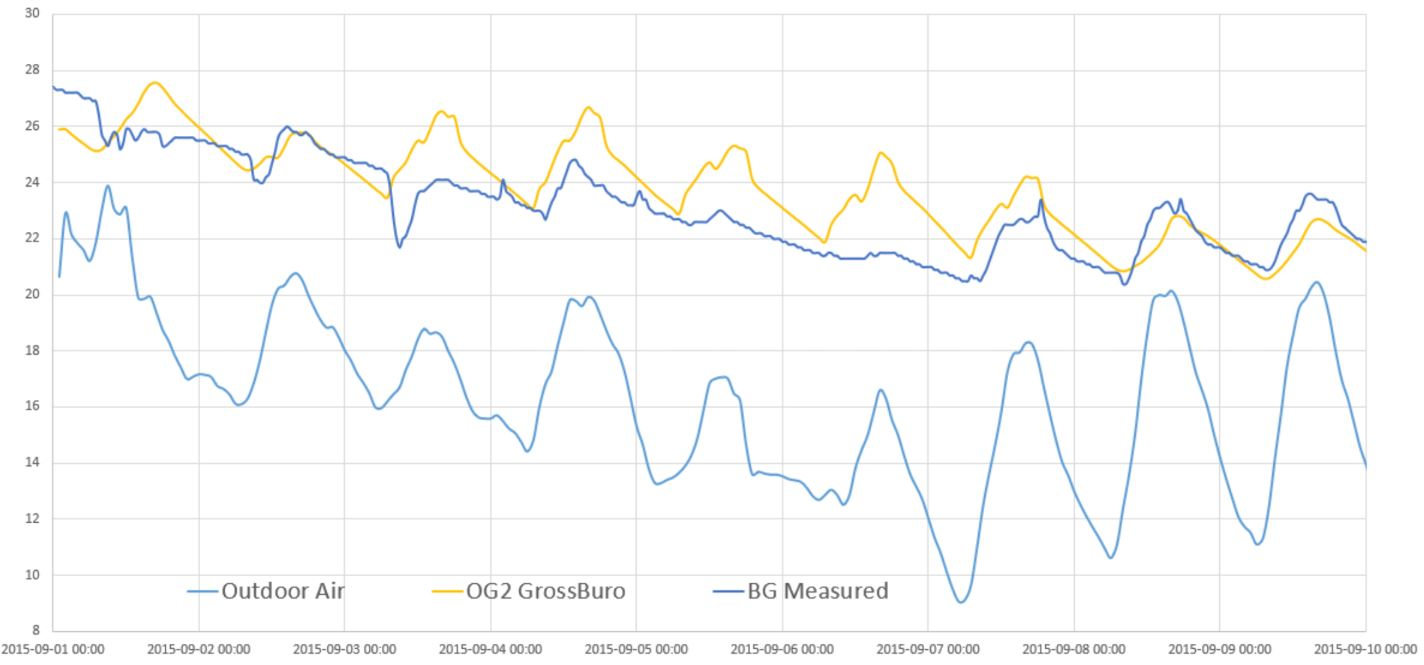
\includegraphics[scale=0.3]{Sumatra_Calibration_AllonShading.JPG}
			\caption{Temperature Profile of Office Building with 24/7 shading}
			\label{fig:Sumatra_Calibration_Allshade}
			\end{figure}			
			
			Table \ref{tab:HonggShadingCtrl} below shows a new shading control schedule in both summer and winter. Another simulation is taken after the new shading schedule is applied on the model. The result in Figure \ref{fig:Sumatra_Calibration_NewShading} below shows an identical pattern as Figure \ref{fig:Sumatra_Calibration_Allshade} in summer period. The annual heating demand for office building with different air infiltration and total ventilation level is shown below at Table \ref{tab:SumatraVentLevel}. As the measured total heating consumption was around 70 $kWh/m^2$, the air infiltration is then calibrated to 0.1 ACH.\\
			
		\begin{table}[htbp]
		\centering
		\caption{New Shading Control Schedule}
		    \begin{tabular}{ccc}
		    \toprule
		    Blind Schedule & Summer & Winter\\
		    \midrule
            Weekday & Always on & 10:00 - 16:00 \\
            Weekend & Always on & Always off\\
		    \bottomrule
		    \end{tabular}%
		  \label{tab:HonggShadingCtrl}%
		\end{table}%
            
            
		\begin{table}[htbp]
		\centering
		\caption{Annual Heating Demand of Office Building in Different Ventilation Level}
		    \begin{tabular}{ccc}
		    \toprule
		    Infiltration Level (ACH) & Total Outdoor Air (ACH) & Heating Demand ($kWh/m^2$)\\
		    \midrule
            0.1 & $\approx$ 0.87 & 71.87\\
            0.2 & $\approx$ 0.97 & 77.97\\
            0.3 & $\approx$ 1.07 & 84.18\\
            
		    \bottomrule
		    \end{tabular}%
		  \label{tab:SumatraVentLevel}%
		\end{table}%
		
		
            \begin{figure}[H]
			\centering
			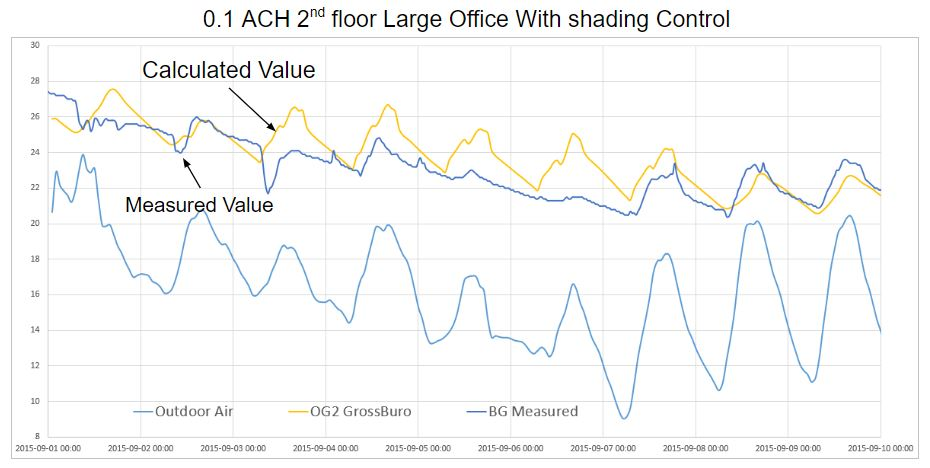
\includegraphics[scale=0.5]{Sumatra_Calibration_NewShading.JPG}
			\caption{Temperature Profile of Office Building with new shading schedule}
			\label{fig:Sumatra_Calibration_NewShading}
			\end{figure}
			
	\section{Parameters Variation Results}

		The parameters variation processes can be done after the buildings are calibrated. The results are presented in a form of histograms and correlation matrices. The histogram helps understand the range of the varied samples and the total influence to parameter variation, while the correlation matrix can better understand the correlations between parameters and parameters, or parameters and heating demand. In addition, the relationship between all parameters and the domestic hot water consumption is also observed from the correlation matrices\\
		
		Figure \ref{fig:Sumatra_StationHistogram} and Figure \ref{fig:Hongg_StationHistogram} below showed the heating demand histograms of the office building and the residential building. The office building has a heating demand range between 55 and 86 $kWh/m^2$ and the residential has a heating demand range between 48 to 68 $kWh/m^2$.\\

	    \begin{figure}[H]
		\centering
		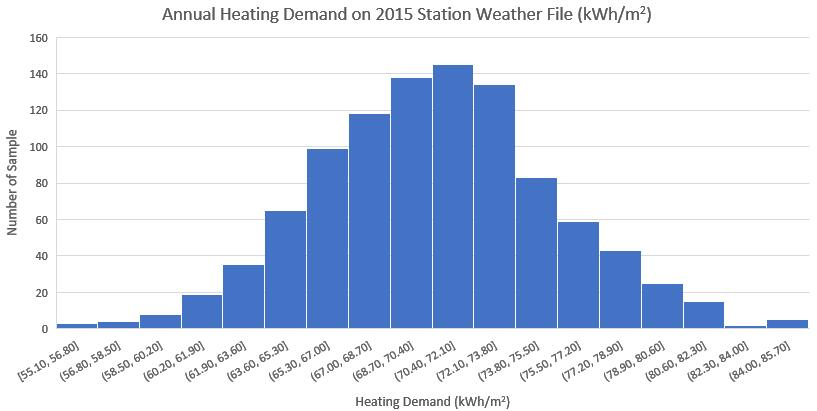
\includegraphics[scale=0.65]{Sumatra_2015Distribution.jpg}
		\caption{Office Building Heating Demand Histogram}
		\label{fig:Sumatra_StationHistogram}
		\end{figure}	

	    \begin{figure}[H]
		\centering
		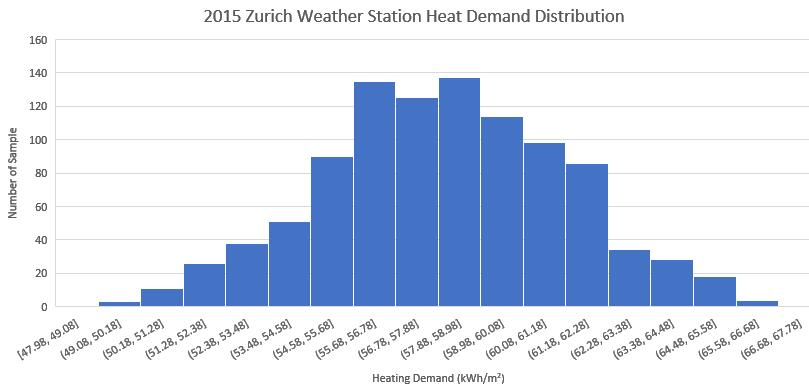
\includegraphics[scale=0.7]{Hongg_2015Distribution.jpg}
		\caption{Residential Building Heating Demand Histogram}
		\label{fig:Hongg_StationHistogram}
		\end{figure}

		Figure \ref{fig:Sumatra_Matrix} and Figure \ref{fig:Hongg_Matrix} below shows the correlation matrices of the office building and the residential building. Correlation matrix is a heat map with many pixels, where each pixel represent a correlation between two intersec parameters. A pixel with deep color indicates the correlation between two parameters is strong, while a pixel with light color indicates the correlation between two parameters is weak.\\
		
		In this thesis, the main focus is the correlation between heating demand, domestic hot water consumption and others. Therefore, the second last row represents the correlation between domestic hot waters and other parameters, and the last row represents the correlation between heating demand and other parameters.\\
		
		The correlation matrix of office building indicates that a strong correlation exists between office temperature setpoint (0.67)/solar absorptance (-0.34) and heating demand. Also, corridor temperature setpoint (0.28) and office appliance (-0.17) are the influential facters among all others. The residential building's correlation matrix also indicated that the key area setpoint temperature (0.58) and the solar absorptance (-0.45) are the influential facters to heating demand. In addition, air infiltration in residential building also showed a very strong correlation of 0.53, making it the second most strongest correlated factor among all. As for domestic hot water, both correlation matrices showed that the domestic hot water demand is strongly depended on the domestic hot water demand of the key area.

		
	    \begin{figure}[H]
		\centering
		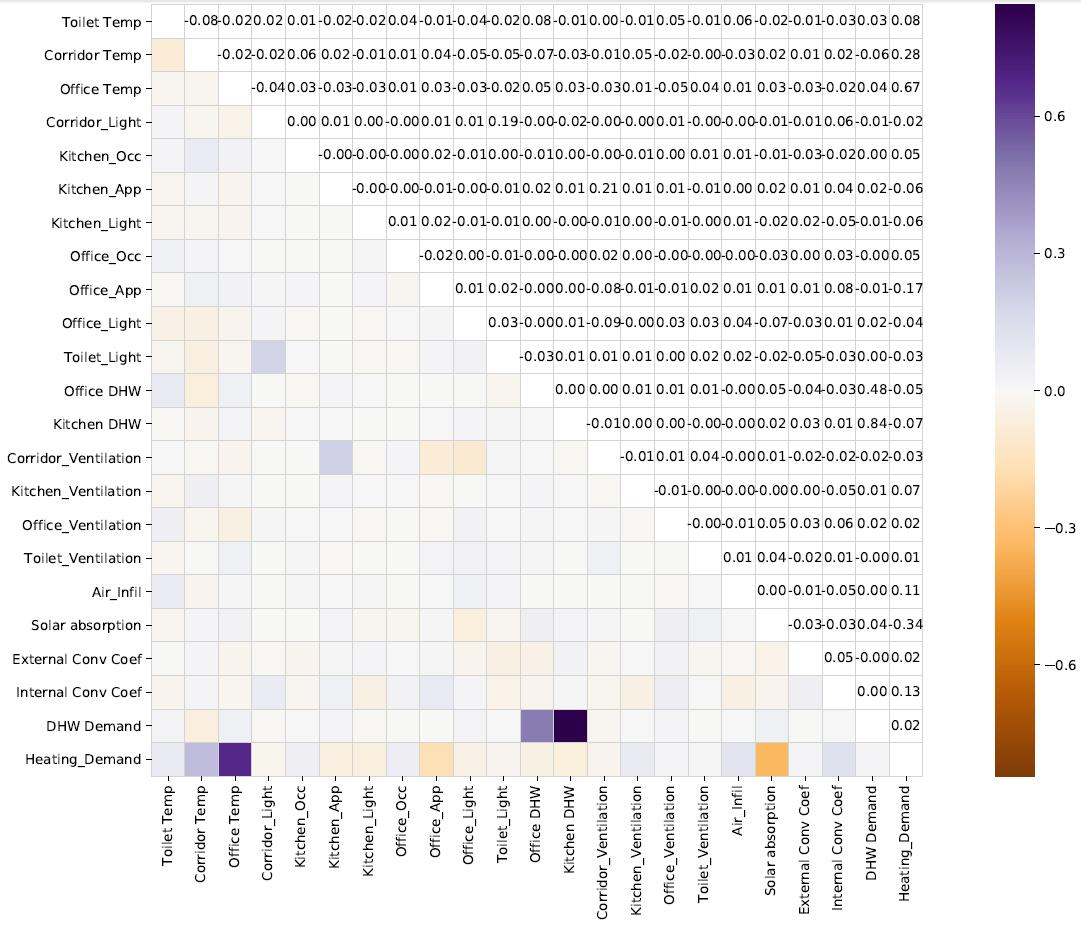
\includegraphics[scale=0.6]{Sumatra_Matrix.jpg}
		\caption{Office Building Correlation Matrix}
		\label{fig:Sumatra_Matrix}
		\end{figure}
			
	    \begin{figure}[H]
		\centering
		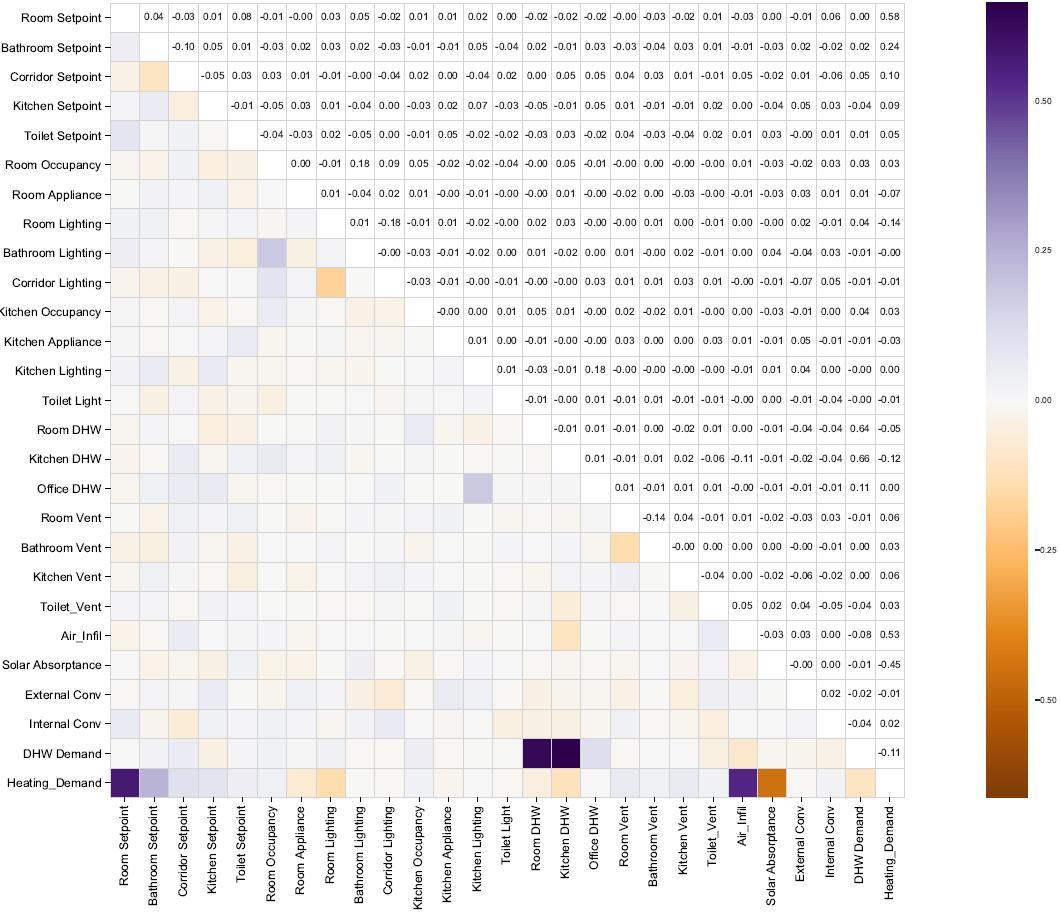
\includegraphics[scale=0.6]{Hongger_Matrix.jpg}
		\caption{Residential Building Correlation Matrix}
		\label{fig:Hongg_Matrix}
		\end{figure}


  	
    \section{Effect of Solar Absorptance on Heating Demand}
			Similarly, an extra set of samples with different solar absorptance are processed in jE-Plus and the results are displayed at the histogram below.\\
			
    	    \begin{figure}[htbp]
    		\centering
    		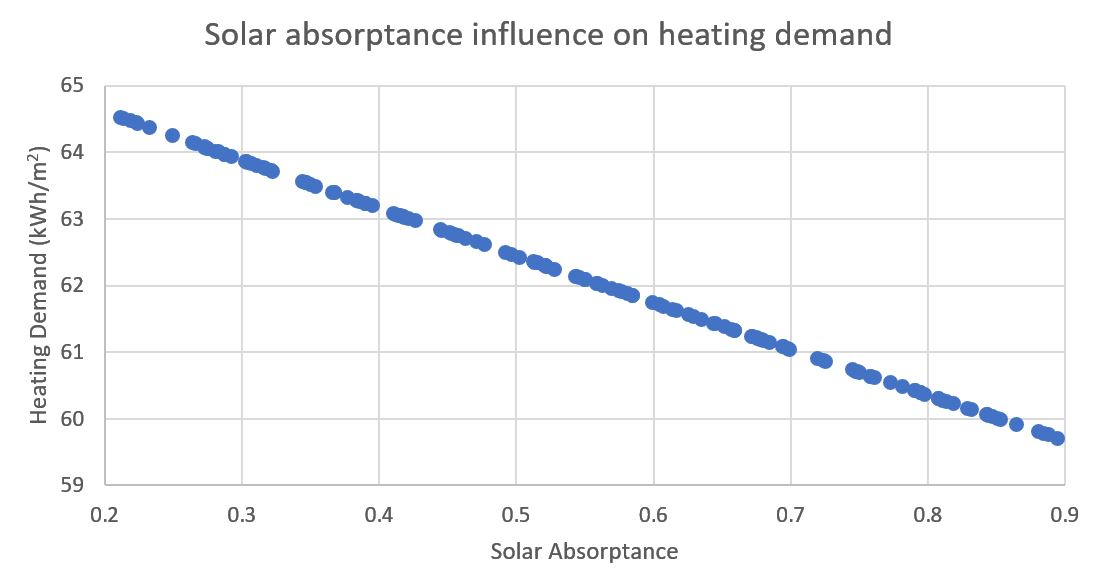
\includegraphics[scale=0.5]{Solar_HeatingDemand.JPG}
    		\caption{Solar Absorptance Influence on Heating Demand (Residential Building)}
    		\label{fig:Hongg_solar}
    		\end{figure}			
        
        The results above show that solar absorptance has proven its ability to influence the heating demand. By solely changing the solar absorptance, the heating demand can achieve a $\pm 4\%$ variation on residential building and $\pm What \%$ in office buildling. Noted that the total variation for $50\%$ of 1000 parameter variation samples is only $\pm 3.4\%$ in the residential building, and $\pm shenme \%$ in the office building (from Figure \ref{fig:Sumatra_Comp}).

	\section{Effect of Convection Coefficient on Heating Demand}
        	As the correlation matrix above indicates a weak correlation between heating demand and heat convection coefficients, which is contradicted to the hypothesis that heat convection coefficient is an important factor in heating demand calculation, another set of simulation with 150 extra samples are processed. These samples are modified from the calibrated building model, with the only difference in convection coefficient (ranging from 90\% to 110\% of the calibrated values). The results are shown in the Figure below. It is clear that $\pm 10\%$ of the heat convection coefficient would have less effects on heating demand than the solar absorptance. \\ 
        	
          	\begin{figure}[htbp]
    		\centering
    		\includegraphics[scale=0.5]{Hongg}
    		\caption{Solar Absorptance Influence on Heating Demand (Residential Building)}
    		\label{fig:Hongg_solar}
    		\end{figure}
        
        \subsection{Global Warming and Heat Island Effect}
		Figure \ref{fig:Sumatra_Comp} and \ref{fig:Hongg_Comp} shows the heating demand range after the parameter variation in three different outdoor environments, namely, the SIA standard hourly data, the 2015 station weather, and the generated heat island weather based on the 2015 station weather. The annual heating demand range shows a clear decline as the outdoor environment gets warmer.

	    \begin{figure}[H]
		\centering
		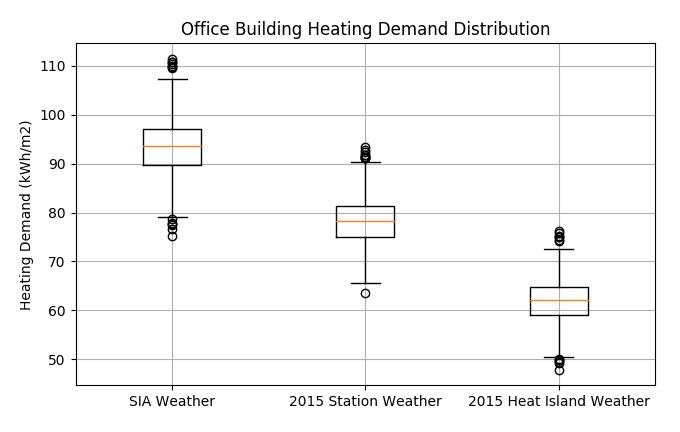
\includegraphics[scale=0.63]{Sumatra_Comparison.jpg}
		\caption{Office Building Heating Demand Comparison}
		\label{fig:Sumatra_Comp}
		\end{figure}

	    \begin{figure}[H]
		\centering
		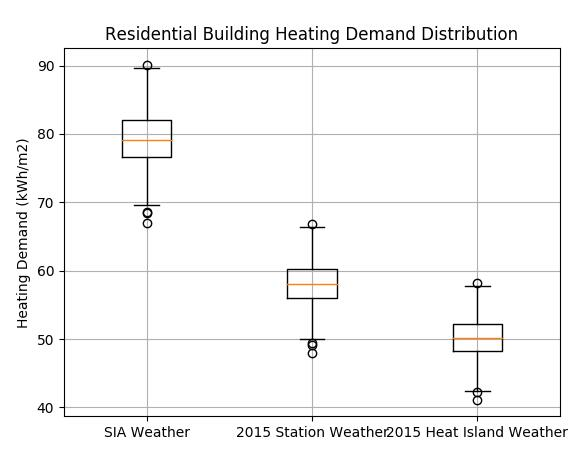
\includegraphics[scale=0.63]{Hongg_Comparison.jpg}
		\caption{Residential Building Heating Demand Comparison}
		\label{fig:Hongg_Comp}
		\end{figure}
		